\documentclass[12pt,a4paper]{article}
\usepackage[utf8]{inputenc}
\usepackage{amsmath}
\usepackage{amsfonts}
\usepackage{amssymb}
\usepackage{graphicx}
\usepackage{geometry}
\usepackage{listings}
\usepackage{xcolor}
\usepackage{hyperref}
\usepackage{tikz}
\usepackage{forest}
\usepackage{underscore}
\usepackage{titlesec}
\usepackage{float}

\usetikzlibrary{shapes,arrows,positioning,calc}

\geometry{margin=0.8in}

% Define colors for the hierarchy
\definecolor{lightblue}{RGB}{173,216,230}
\definecolor{lightgreen}{RGB}{144,238,144}
\definecolor{lightgray}{RGB}{211,211,211}
\definecolor{lightcyan}{RGB}{224,255,255}
\definecolor{wheat}{RGB}{245,222,179}

% Fix heading alignment and hierarchy
\titleformat{\section}{\Large\bfseries}{\thesection}{1em}{}
\titleformat{\subsection}{\large\bfseries}{\thesubsection}{1em}{}
\titlespacing*{\section}{0pt}{3.5ex plus 1ex minus .2ex}{2.3ex plus .2ex}
\titlespacing*{\subsection}{0pt}{3.25ex plus 1ex minus .2ex}{1.5ex plus .2ex}

% Define UML styles
\tikzset{
    umlclass/.style={
        rectangle,
        draw=black,
        minimum width=3cm,
        minimum height=1cm,
        text centered,
        font=\small
    },
    inheritance/.style={
        ->,
        >=open triangle 45,
        thick
    }
}

% Code listing style
\lstset{
    language=C++,
    basicstyle=\ttfamily\small,
    keywordstyle=\color{blue},
    commentstyle=\color{green},
    stringstyle=\color{red},
    numberstyle=\tiny\color{gray},
    numbers=left,
    frame=single,
    breaklines=true,
    tabsize=4
}

\title{Data Abstraction and Object Orientation \\ (CSF301 Assignment)}
\author{Pranav M R, Arinjay Jain, Kanishk Rai, Anshul Rakesh}
\date{September 18, 2025}

\begin{document}

\maketitle
\tableofcontents
\newpage

\section{Class Hierarchy Overview}

The design follows a clear inheritance structure with \texttt{AbstractList} as the root abstract class, providing fundamental list operations. The hierarchy branches into three main categories:

\begin{enumerate}
    \item \textbf{Stack}: Direct concrete implementation of LIFO behavior
    \item \textbf{Queue}: FIFO behavior with extensions for priority and deque functionality  
    \item \textbf{TraversableList}: Lists that support iteration and indexing, with array and linked implementations
\end{enumerate}

\section{Class Hierarchy Flowchart}

\begin{figure}[H]
\centering
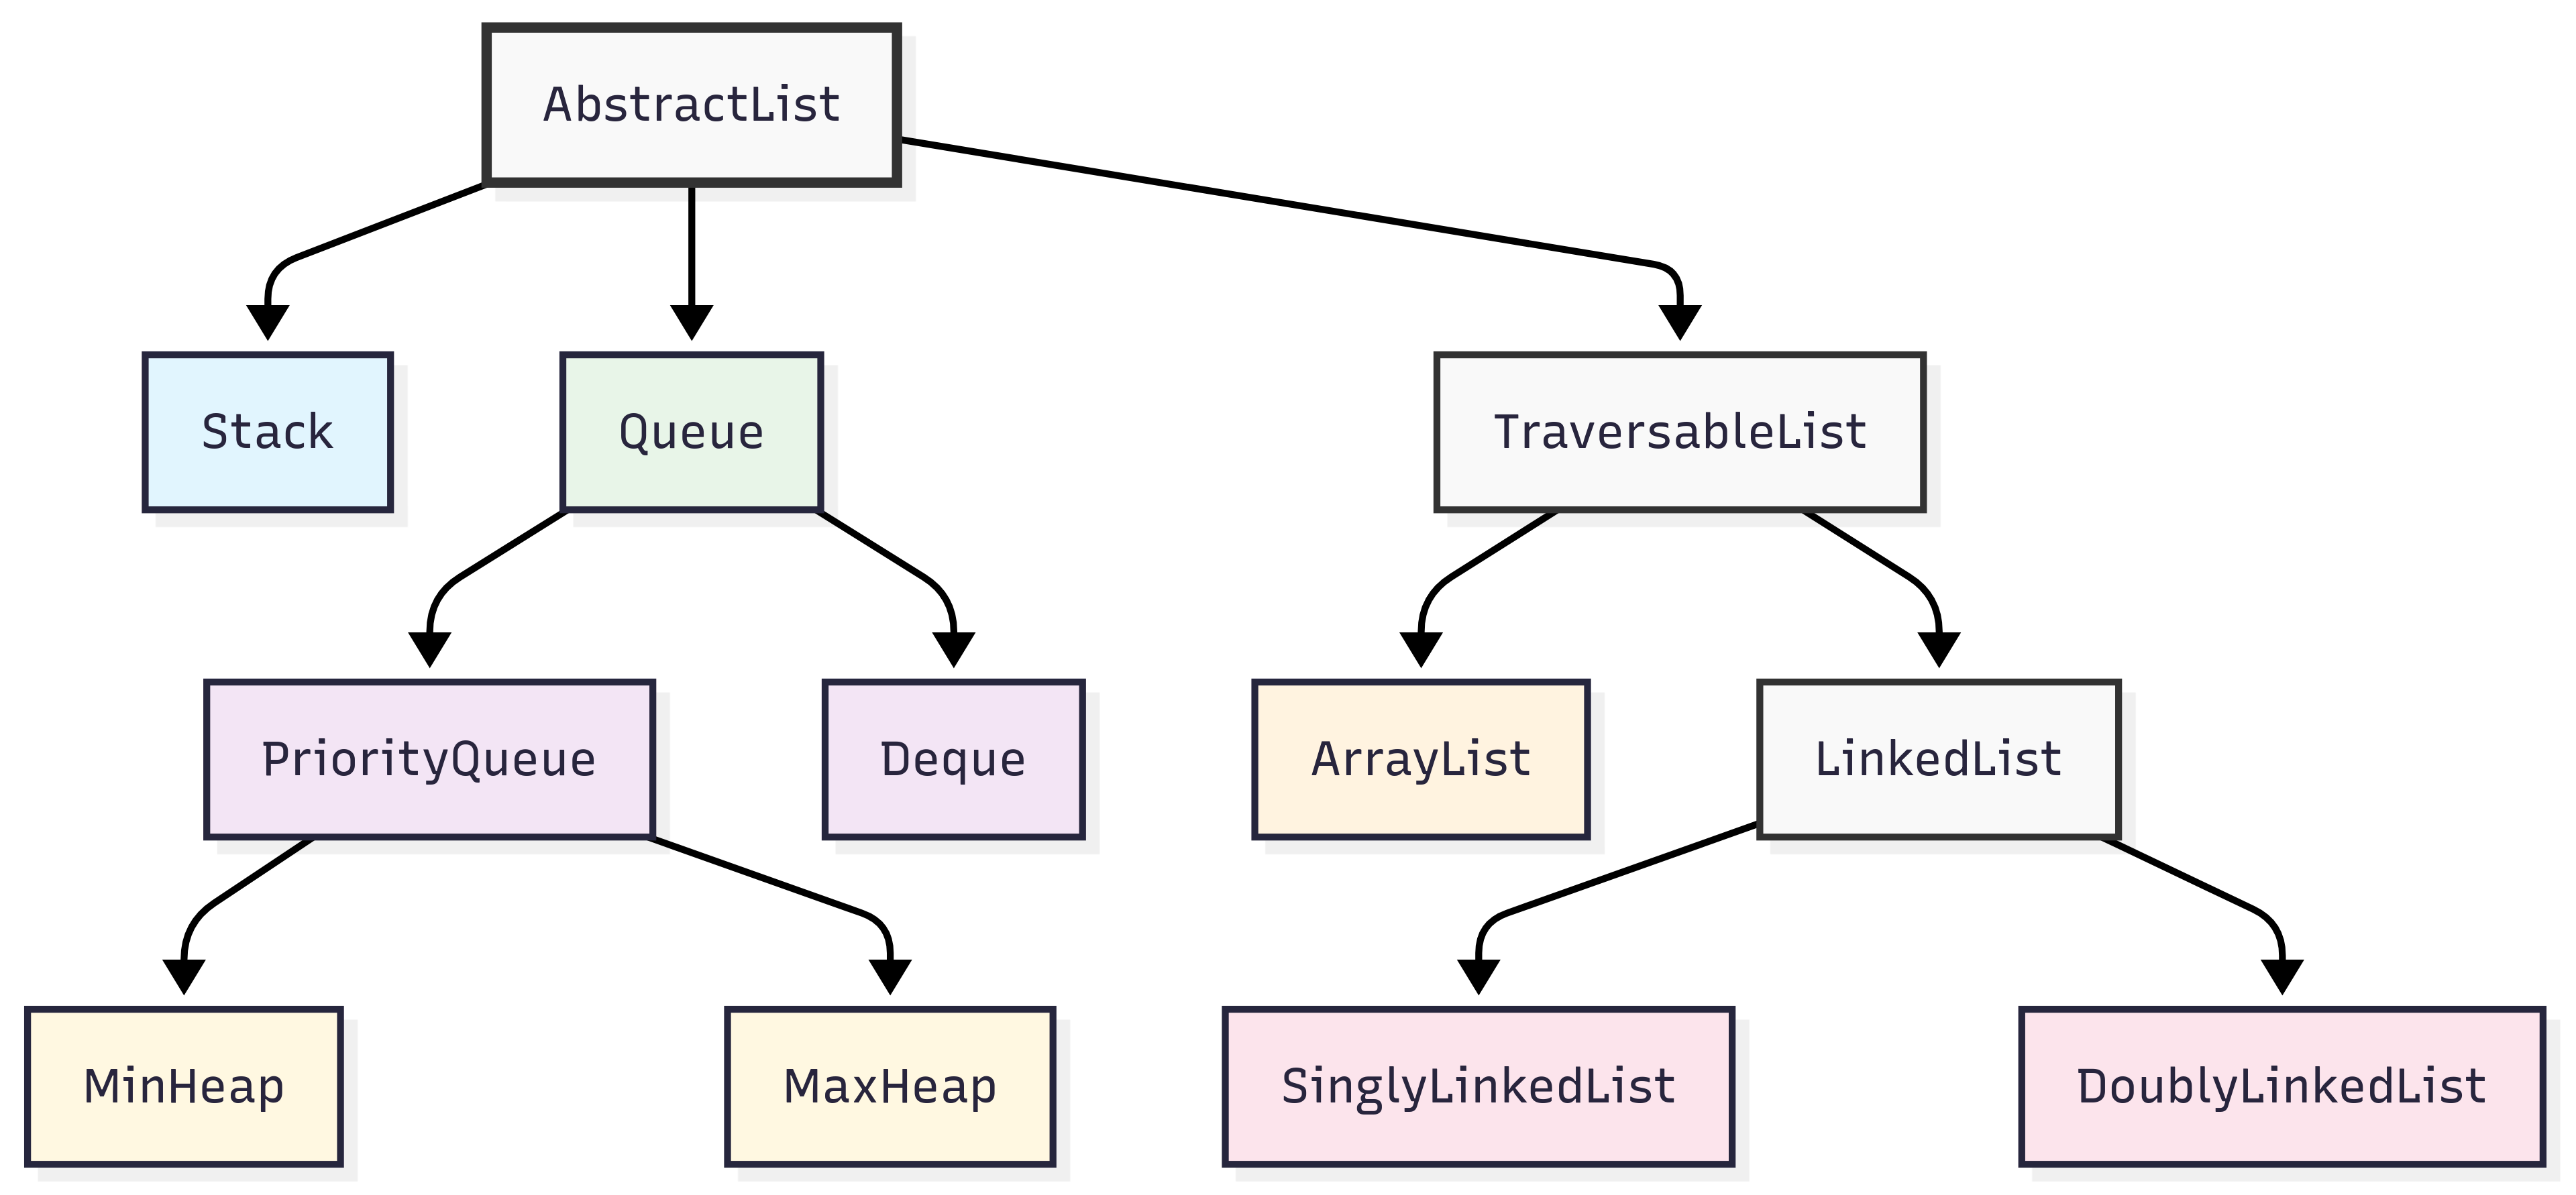
\includegraphics[width=0.9\textwidth]{figures/1.png}
\caption{Complete Class Hierarchy Structure}
\label{fig:hierarchy}
\end{figure}

\section{UML Class Diagrams}

\subsection{Stack Implementation}

\begin{figure}[H]
\centering
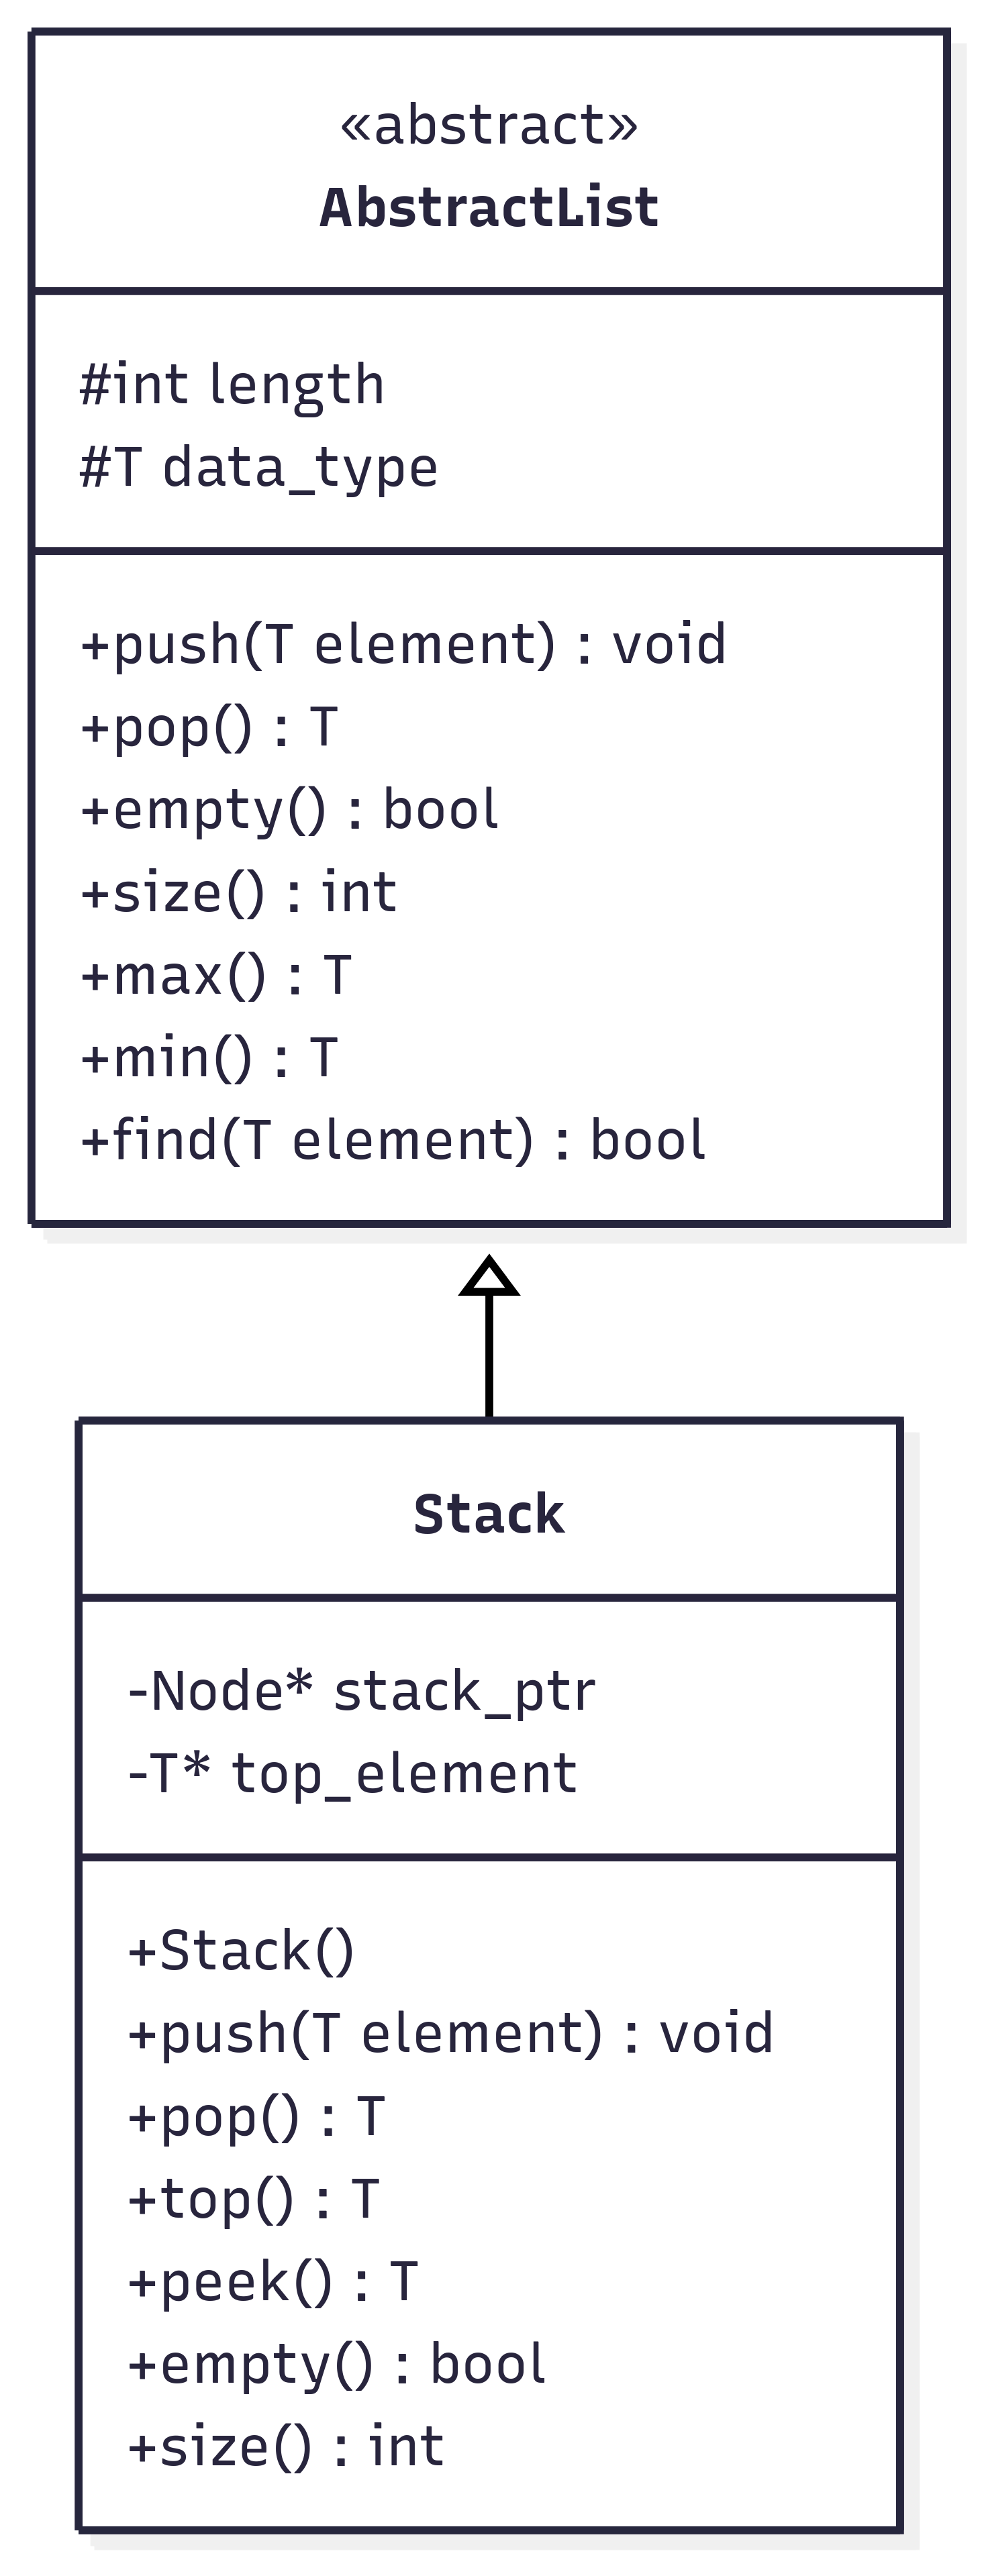
\includegraphics[width=0.25\textwidth]{figures/3.png}
\caption{Stack Class Inheritance}
\label{fig:stack-inheritance}
\end{figure}

The Stack class provides a Last-In-First-Out (LIFO) data structure implementation. It inherits from AbstractList and specializes the push/pop operations to work exclusively with the top of the stack.

\textbf{Key Design Features:}
\begin{itemize}
    \item \textbf{Single Access Point}: All operations occur at the top of the stack
    \item \textbf{Node-Based Storage}: Uses linked nodes for dynamic sizing
    \item \textbf{Top Element Caching}: Maintains a pointer to the top element for O(1) access
    \item \textbf{Exception Safety}: Throws underflow exceptions when popping from empty stack
\end{itemize}

\textbf{Memory Management:}
\begin{itemize}
    \item Dynamic allocation/deallocation of nodes
    \item Automatic cleanup in destructor
    \item No memory leaks through proper node management
\end{itemize}

\subsection{Queue Family}

\begin{figure}[H]
\centering
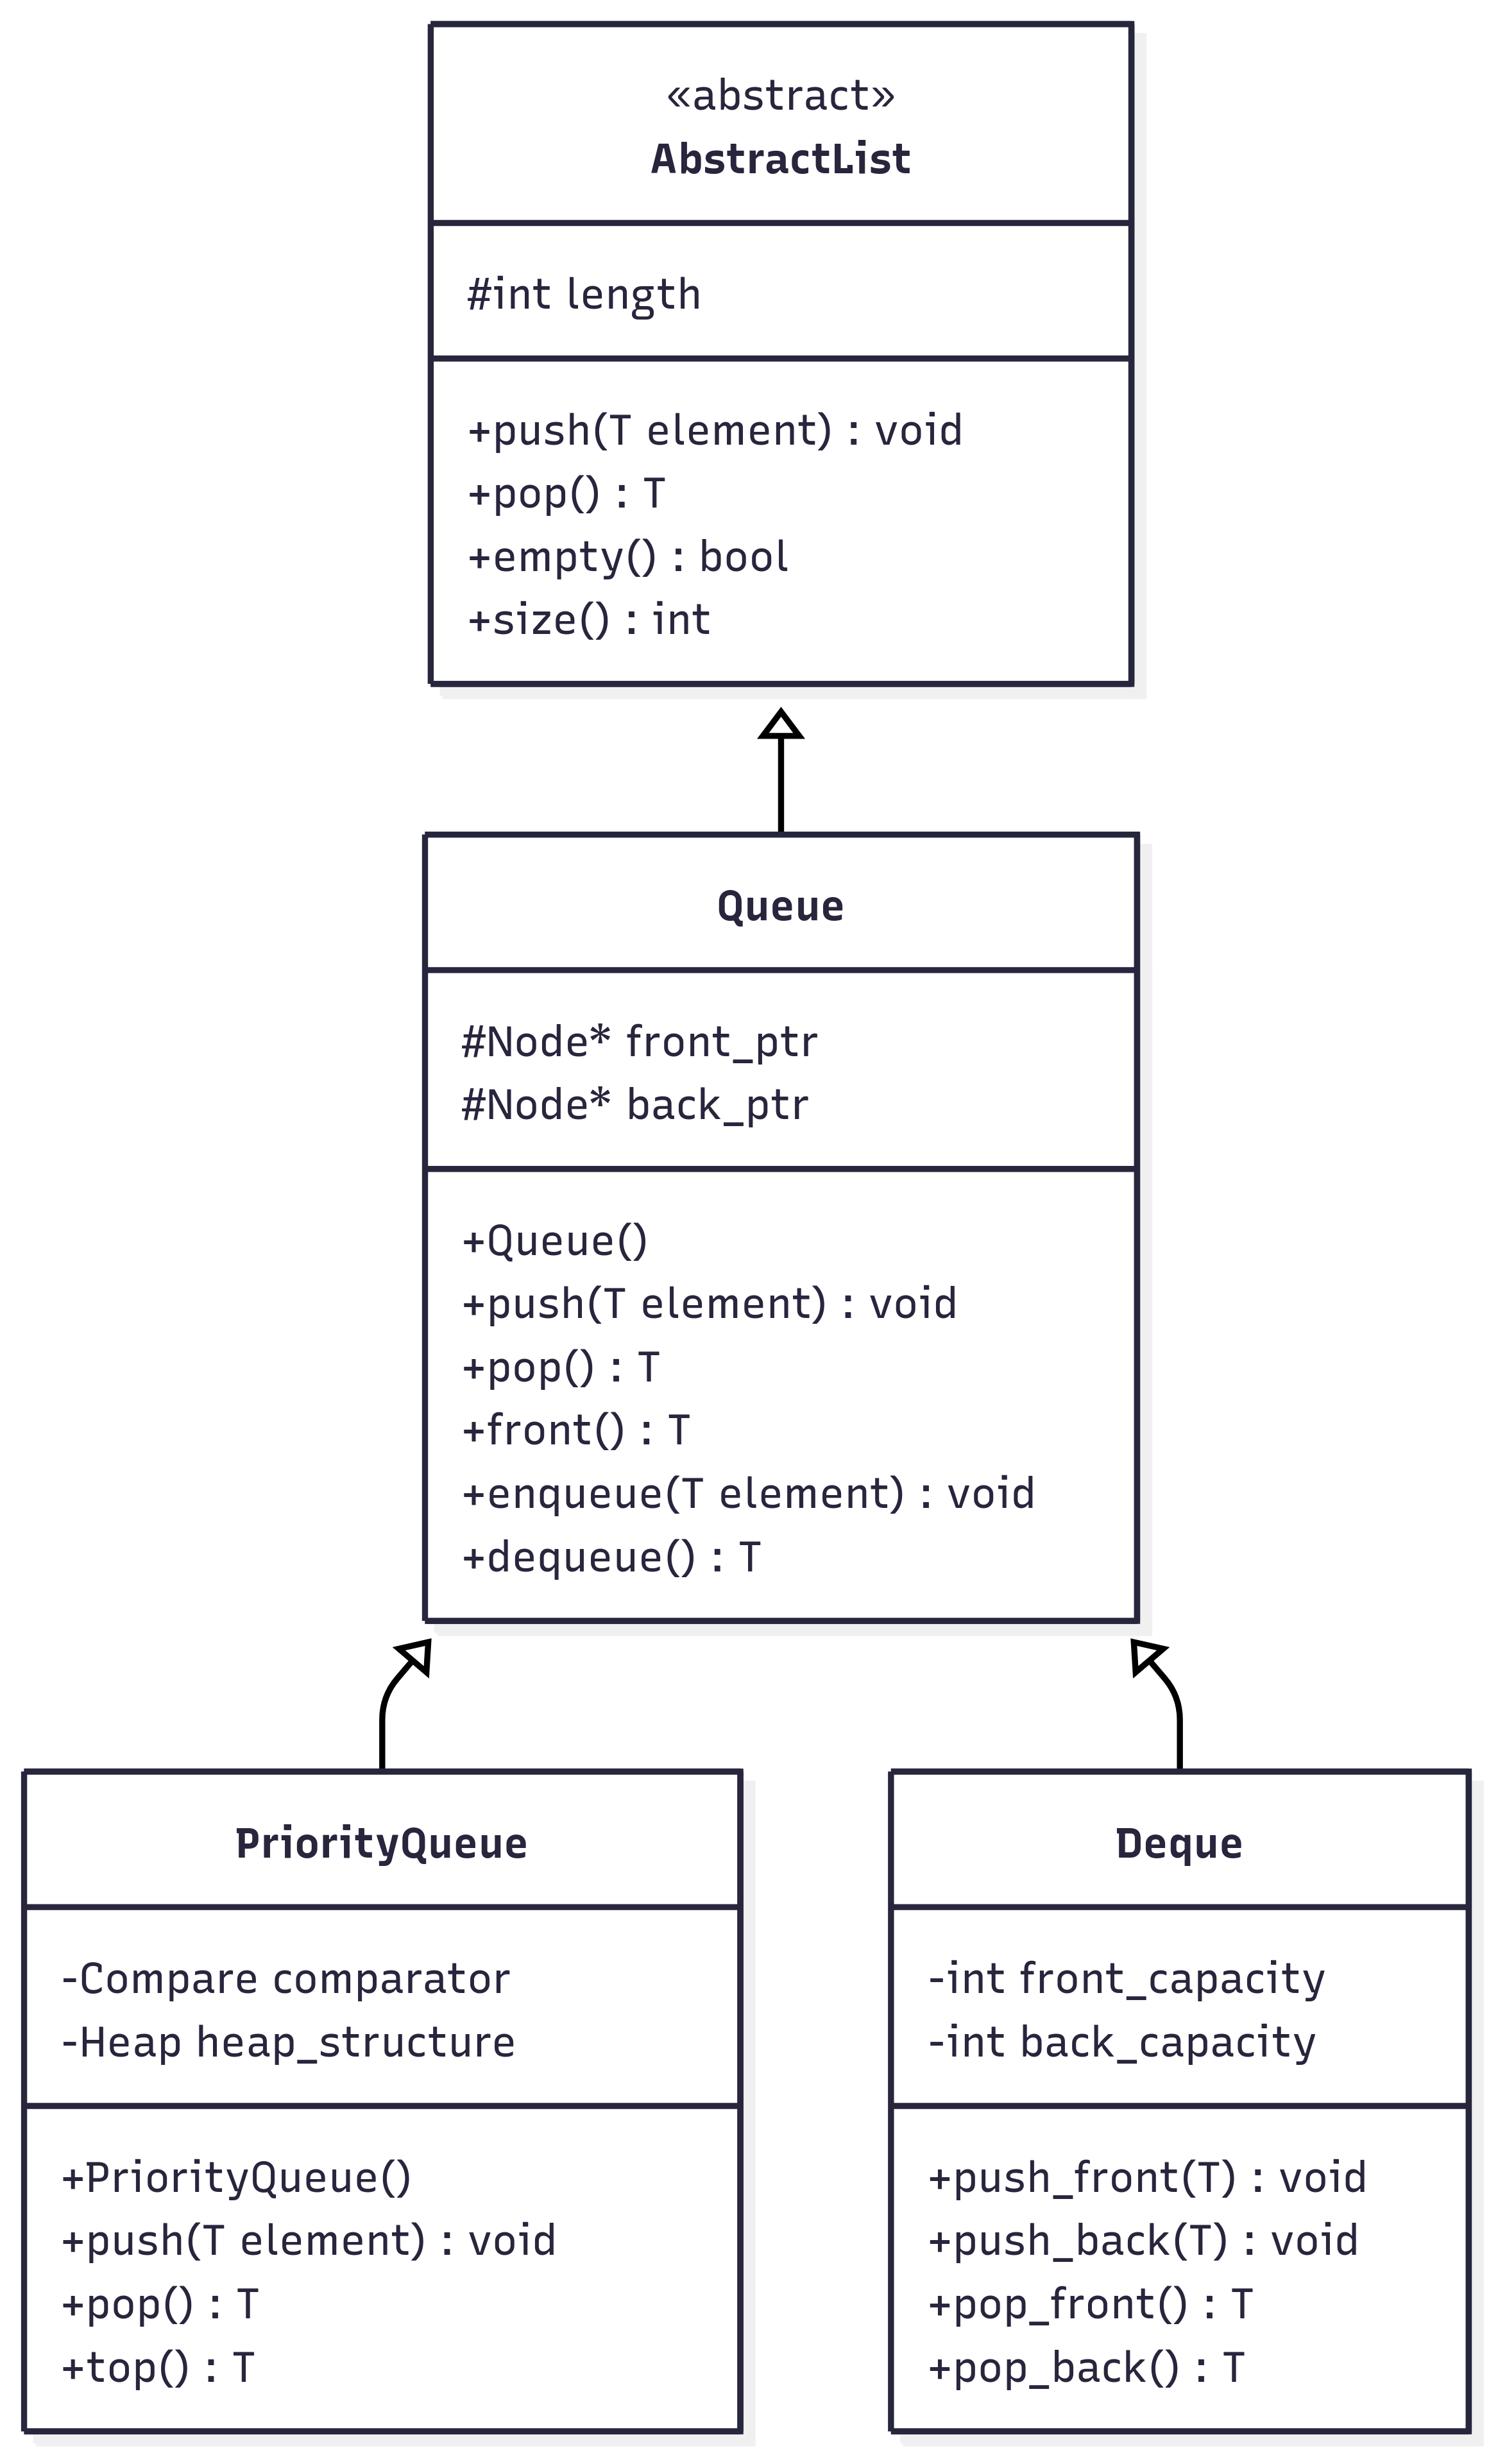
\includegraphics[width=0.35\textwidth]{figures/4.png}
\caption{Queue Family Class Hierarchy}
\label{fig:queue-family}
\end{figure}

The Queue family implements First-In-First-Out (FIFO) data structures with various specializations for different use cases.

\textbf{Base Queue Features:}
\begin{itemize}
    \item \textbf{Dual-Pointer Design}: Maintains separate front and back pointers for O(1) operations
    \item \textbf{FIFO Semantics}: Elements added at back, removed from front
    \item \textbf{Flexible Interface}: Supports both push/pop and enqueue/dequeue terminology
\end{itemize}

\textbf{PriorityQueue Specialization:}
\begin{itemize}
    \item \textbf{Heap-Based Implementation}: Uses binary heap for efficient priority ordering
    \item \textbf{Customizable Comparator}: Allows user-defined priority functions
    \item \textbf{Logarithmic Complexity}: O(log n) insertion and removal
    \item \textbf{Constant Top Access}: O(1) access to highest priority element
\end{itemize}

\textbf{Deque Capabilities:}
\begin{itemize}
    \item \textbf{Double-Ended Operations}: Insertion and removal at both ends
    \item \textbf{Capacity Management}: Tracks available space at front and back
    \item \textbf{Versatile Usage}: Can function as both stack and queue
    \item \textbf{Optimized Storage}: Circular buffer implementation for space efficiency
\end{itemize}

\subsection{TraversableList Family}

\begin{figure}[H]
\centering
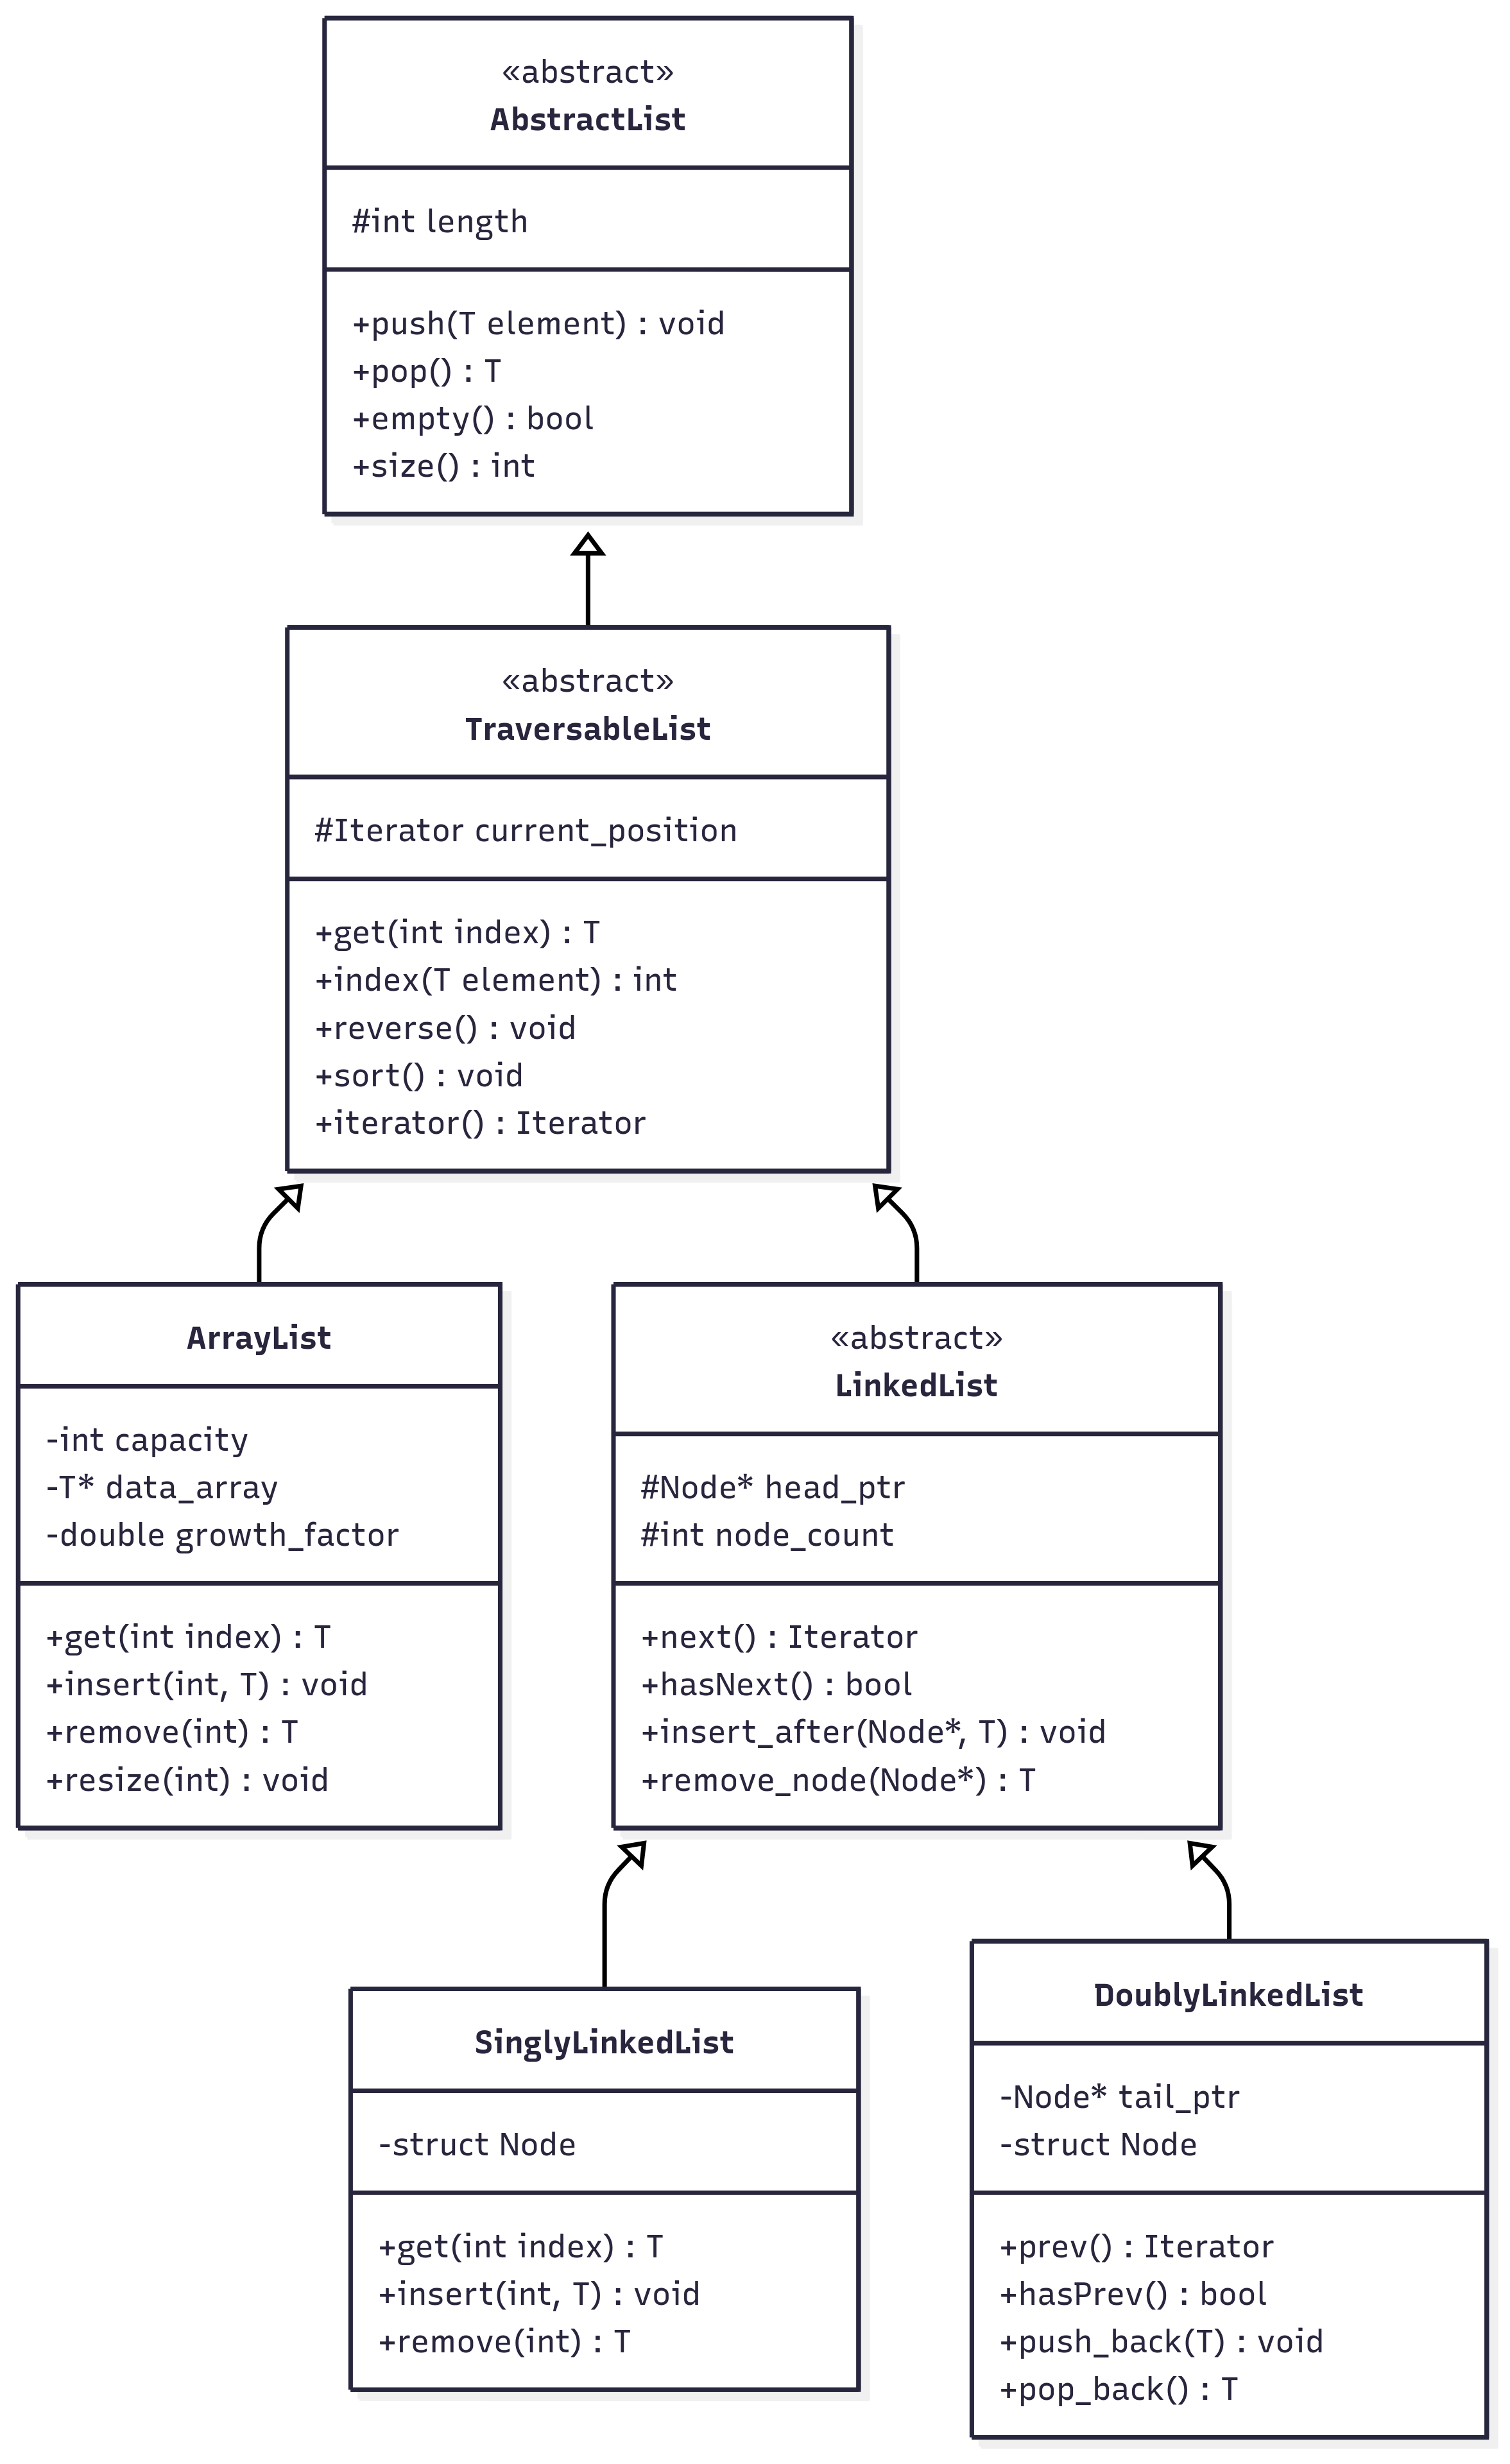
\includegraphics[width=0.4\textwidth]{figures/5.png}
\caption{TraversableList Family Class Hierarchy}
\label{fig:traversable-family}
\end{figure}

The TraversableList family provides indexed access and iteration capabilities, implementing two fundamental storage strategies: array-based and linked-node-based.

\textbf{TraversableList Abstract Features:}
\begin{itemize}
    \item \textbf{Iterator Pattern Implementation}: Provides standard iteration interface
    \item \textbf{Random Access Support}: Get/set elements by index
    \item \textbf{Sorting Capabilities}: Built-in sort with customizable comparators
    \item \textbf{Reversal Operations}: In-place list reversal
    \item \textbf{Search Functionality}: Find elements and return indices
\end{itemize}

\textbf{ArrayList Characteristics:}
\begin{itemize}
    \item \textbf{Contiguous Memory}: Array-based storage for cache efficiency
    \item \textbf{Dynamic Resizing}: Automatic capacity expansion with configurable growth factor
    \item \textbf{Random Access}: O(1) indexed access to elements
    \item \textbf{Amortized Performance}: O(1) amortized insertion at end
    \item \textbf{Memory Optimization}: Shrink-to-fit functionality to reduce memory footprint
\end{itemize}

\textbf{LinkedList Family:}

\textit{SinglyLinkedList Features:}
\begin{itemize}
    \item \textbf{Memory Efficient}: Minimal overhead per node (one pointer)
    \item \textbf{Forward Traversal}: Unidirectional iteration capability
    \item \textbf{Dynamic Size}: No pre-allocation required
    \item \textbf{Efficient Head Operations}: O(1) insertion/deletion at beginning
\end{itemize}

\textit{DoublyLinkedList Features:}
\begin{itemize}
    \item \textbf{Bidirectional Traversal}: Forward and backward iteration
    \item \textbf{Tail Pointer Optimization}: O(1) operations at both ends
    \item \textbf{Flexible Navigation}: Previous/next navigation in constant time
    \item \textbf{Enhanced Iterator}: Support for reverse iteration patterns
\end{itemize}

\textbf{Performance Trade-offs:}
\begin{table}[h!]
\centering
\begin{tabular}{|l|c|c|c|}
\hline
\textbf{Operation} & \textbf{ArrayList} & \textbf{SinglyLinked} & \textbf{DoublyLinked} \\
\hline
Random Access & O(1) & O(n) & O(n) \\
Insert at Head & O(n) & O(1) & O(1) \\
Insert at Tail & O(1)* & O(n) & O(1) \\
Insert at Middle & O(n) & O(1)** & O(1)** \\
Memory per Element & Low & Medium & High \\
Cache Performance & Excellent & Poor & Poor \\
\hline
\end{tabular}
\caption{TraversableList Implementation Comparison (*Amortized, **At known position)}
\end{table}

\section{Complete Class Hierarchy Overview}

\begin{figure}[H]
\centering
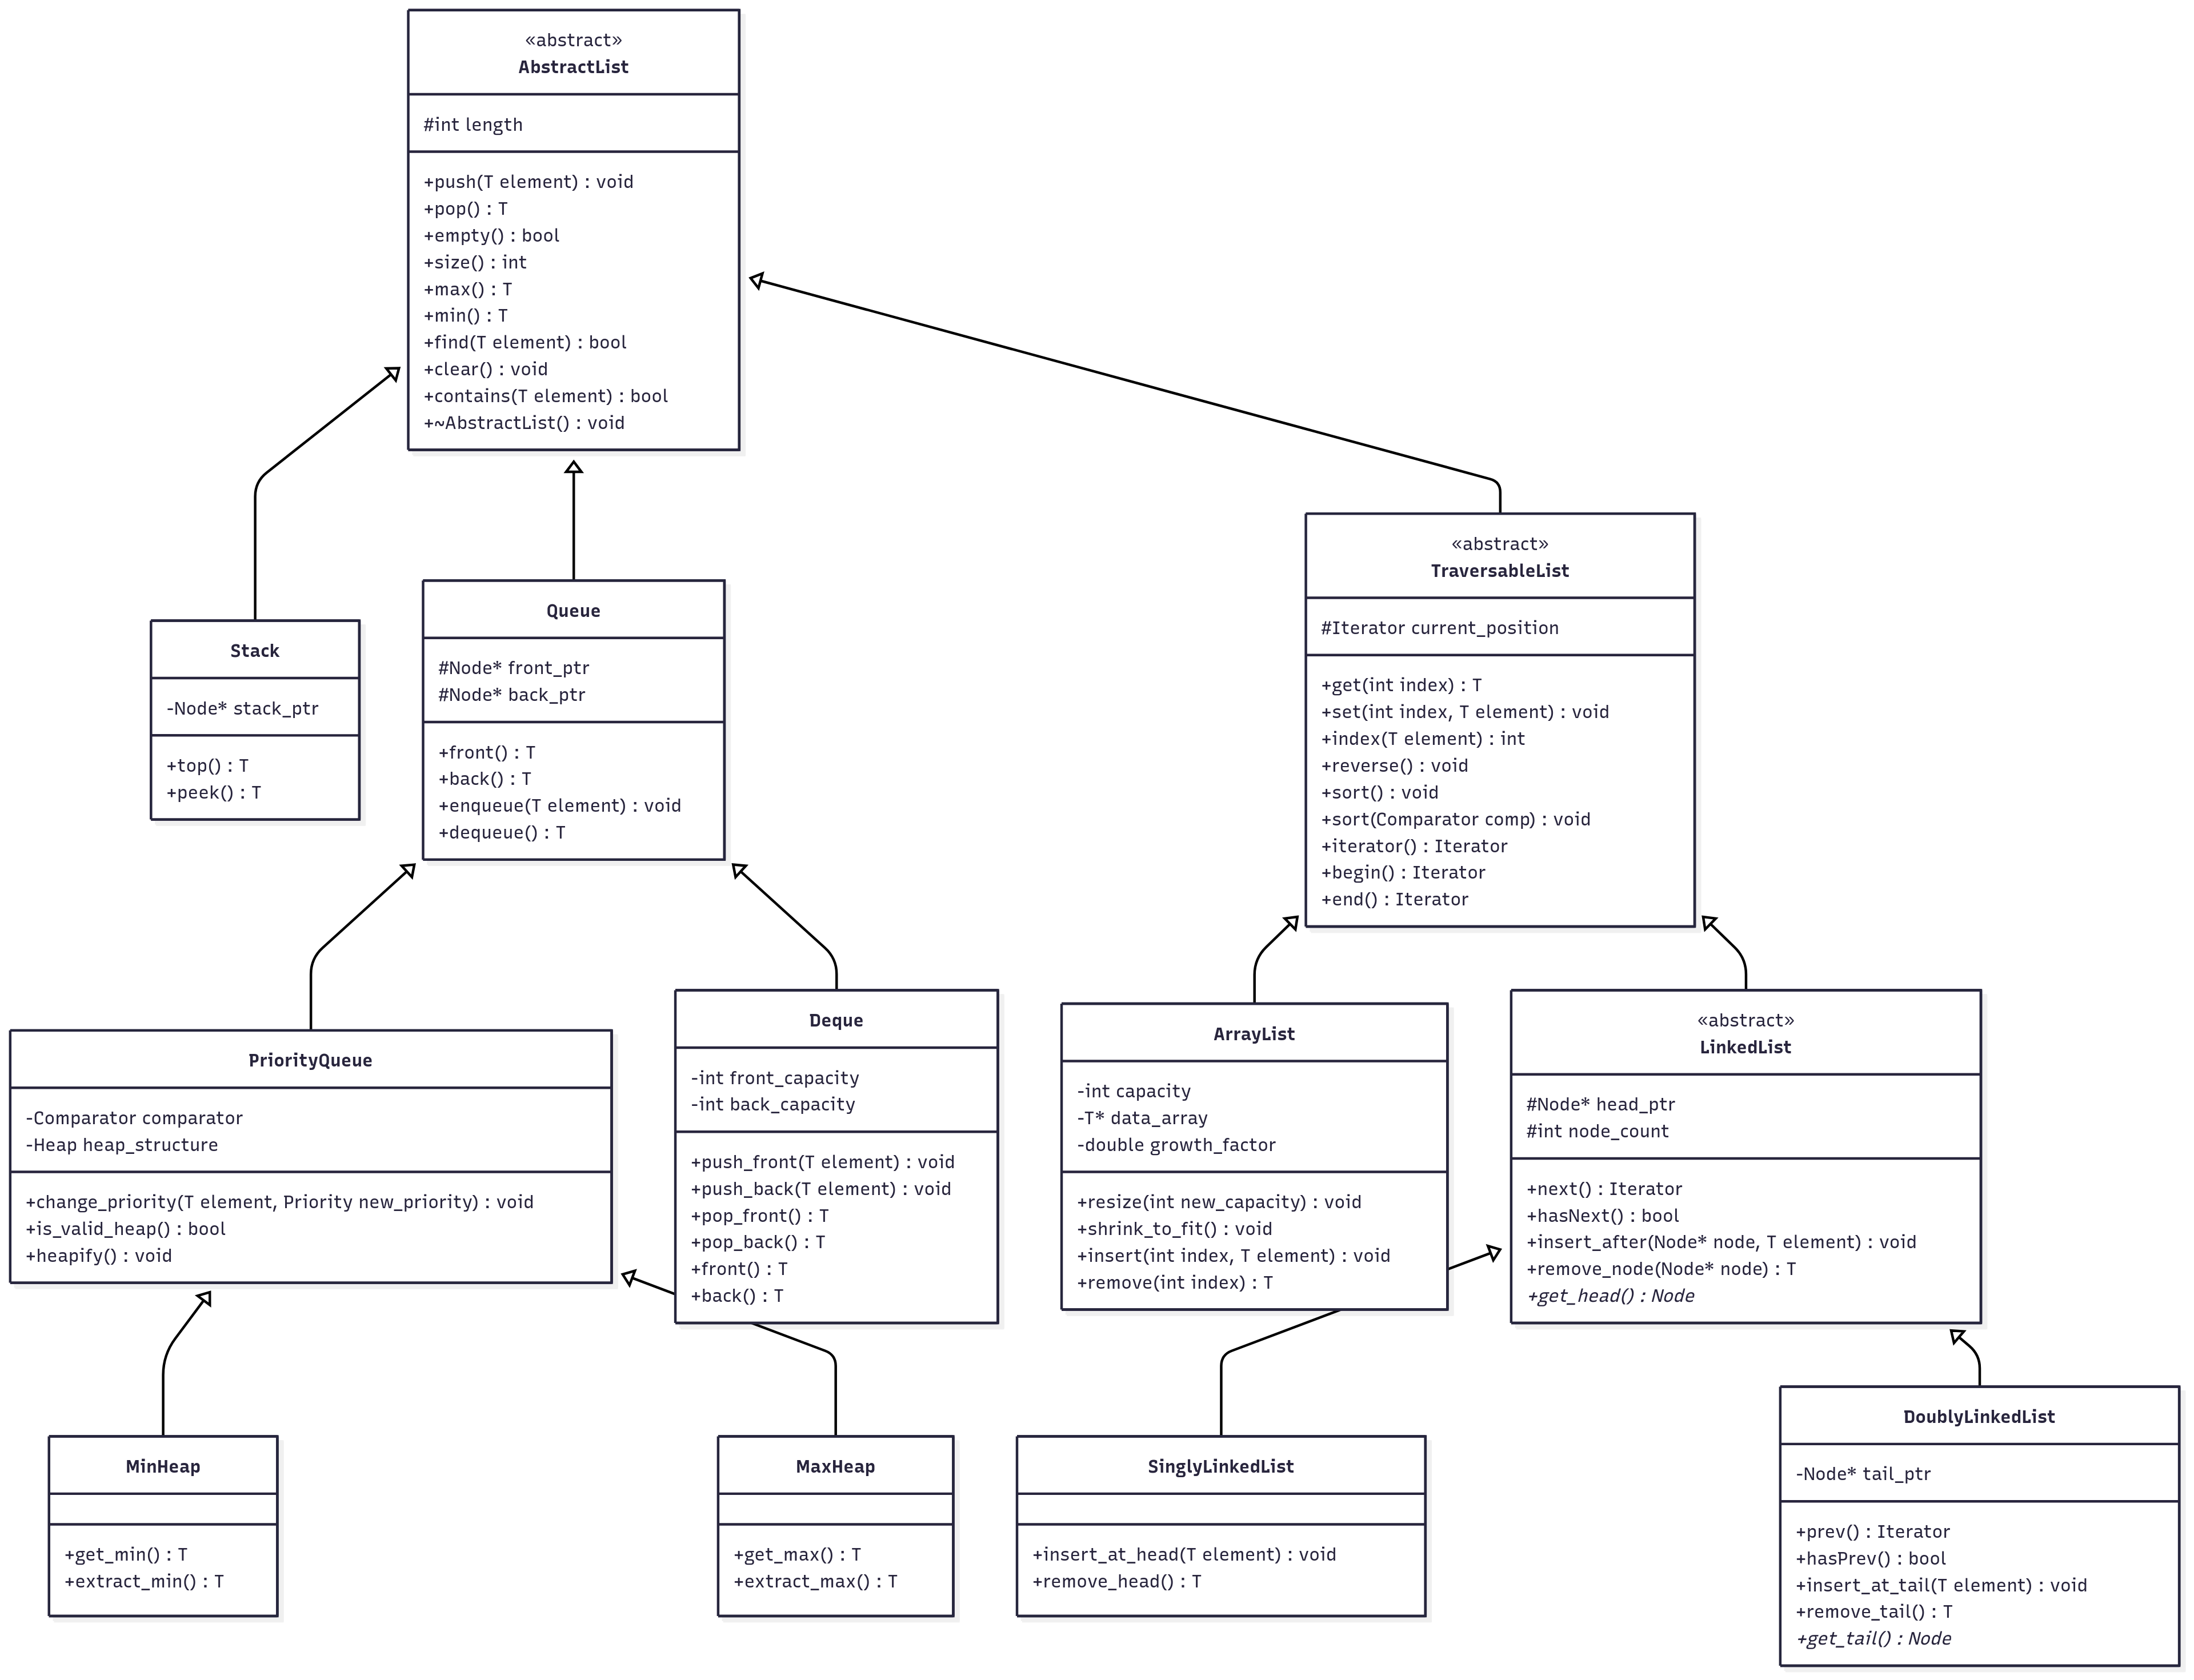
\includegraphics[width=0.9\textwidth]{figures/2.png}
\caption{Complete UML Class Hierarchy with All Relationships}
\label{fig:complete-hierarchy}
\end{figure}

\section{Detailed Class Specifications}

\subsection{AbstractList - Root Abstract Class}

\textbf{Purpose:} Provides fundamental list operations as an interface contract.

\textbf{Attributes:}
\begin{itemize}
    \item \texttt{length}: Current number of elements in the list
    \item \texttt{data\_type}: Template parameter for element type
\end{itemize}

\textbf{Key Methods and API Promises:}
\begin{itemize}
    \item \texttt{push(element)}: Add element to the list (implementation varies by subclass)
    \item \texttt{pop()}: Remove and return an element (implementation varies by subclass)
    \item \texttt{empty()}: Returns true if list has no elements - O(1)
    \item \texttt{size()}: Returns current number of elements - O(1)
    \item \texttt{max()}: Returns maximum element in the list - O(n)
    \item \texttt{min()}: Returns minimum element in the list - O(n)
    \item \texttt{find(element)}: Returns true if element exists - O(n) typical
    \item \texttt{clear()}: Remove all elements - O(n)
\end{itemize}

\subsection{Stack - LIFO Container}

\textbf{Purpose:} Last In, First Out container with top-only access.

\textbf{Additional Attributes:}
\begin{itemize}
    \item \texttt{stack\_ptr}: Pointer to top of stack
    \item \texttt{top\_element}: Cache for top element access
\end{itemize}

\textbf{API Promises:}
\begin{itemize}
    \item \texttt{push(element)}: Add element to top of stack - O(1)
    \item \texttt{pop()}: Remove and return top element - O(1)
    \item \texttt{top()}: Return top element without removing - O(1)
    \item \texttt{peek()}: Alias for top() - O(1)
    \item Throws \texttt{std::underflow\_error} on pop/top when empty
    \item Thread-safe operations (optional extension)
\end{itemize}

\subsection{Queue - FIFO Container}

\textbf{Purpose:} First In, First Out container with front and back access.

\textbf{Additional Attributes:}
\begin{itemize}
    \item \texttt{front\_ptr}: Pointer to front of queue
    \item \texttt{back\_ptr}: Pointer to back of queue
\end{itemize}

\textbf{API Promises:}
\begin{itemize}
    \item \texttt{push(element)}: Add element to back (enqueue) - O(1)
    \item \texttt{pop()}: Remove and return front element (dequeue) - O(1)
    \item \texttt{front()}: Return front element without removing - O(1)
    \item \texttt{enqueue(element)}: Alias for push() - O(1)
    \item \texttt{dequeue()}: Alias for pop() - O(1)
    \item Throws \texttt{std::underflow\_error} on dequeue/front when empty
\end{itemize}

\subsection{PriorityQueue - Priority-Ordered Container}

\textbf{Purpose:} Queue where elements are served based on priority rather than insertion order.

\textbf{Additional Attributes:}
\begin{itemize}
    \item \texttt{comparator}: Function object for element comparison
    \item \texttt{heap\_structure}: Internal heap for maintaining priority order
\end{itemize}

\textbf{API Promises:}
\begin{itemize}
    \item \texttt{push(element)}: Insert maintaining priority order - O(log n)
    \item \texttt{pop()}: Remove and return highest priority element - O(log n)
    \item \texttt{top()}: Return highest priority element - O(1)
    \item \texttt{change\_priority(element, new\_priority)}: Update priority - O(log n)
    \item Customizable comparison function
    \item Stable ordering for equal priorities (optional)
\end{itemize}

\subsection{MinHeap \& MaxHeap - Specialized Priority Queues}

\textbf{Purpose:} Pre-configured priority queues for common use cases.

\textbf{MinHeap API Promises:}
\begin{itemize}
    \item Smallest element has highest priority
    \item \texttt{get\_min()}: Return minimum element - O(1)
    \item All PriorityQueue operations with min-comparator
\end{itemize}

\textbf{MaxHeap API Promises:}
\begin{itemize}
    \item Largest element has highest priority
    \item \texttt{get\_max()}: Return maximum element - O(1)
    \item All PriorityQueue operations with max-comparator
\end{itemize}

\subsection{Deque - Double-Ended Queue}

\textbf{Purpose:} Queue allowing efficient insertion and removal at both ends.

\textbf{Additional Attributes:}
\begin{itemize}
    \item \texttt{front\_capacity}: Available space at front
    \item \texttt{back\_capacity}: Available space at back
\end{itemize}

\textbf{API Promises:}
\begin{itemize}
    \item \texttt{push\_front(element)}: Add element to front - O(1)
    \item \texttt{push\_back(element)}: Add element to back - O(1)
    \item \texttt{pop\_front()}: Remove from front - O(1)
    \item \texttt{pop\_back()}: Remove from back - O(1)
    \item \texttt{front()}: Access front element - O(1)
    \item \texttt{back()}: Access back element - O(1)
    \item Can function as both stack and queue
\end{itemize}

\subsection{TraversableList - Indexable Container}

\textbf{Purpose:} Abstract base for lists supporting indexed access and iteration.

\textbf{Additional Attributes:}
\begin{itemize}
    \item \texttt{current\_position}: Iterator position for traversal
\end{itemize}

\textbf{API Promises:}
\begin{itemize}
    \item \texttt{get(index)}: Return element at specified index
    \item \texttt{index(element)}: Return index of first occurrence
    \item \texttt{reverse()}: Reverse the order of elements
    \item \texttt{sort()}: Sort elements in ascending order
    \item \texttt{sort(comparator)}: Sort with custom comparator
    \item \texttt{iterator()}: Return iterator for traversal
    \item \texttt{begin()}/\texttt{end()}: Standard iterator interface
    \item Support for range-based for loops
\end{itemize}

\subsection{ArrayList - Dynamic Array Implementation}

\textbf{Purpose:} Resizable array with random access capabilities.

\textbf{Additional Attributes:}
\begin{itemize}
    \item \texttt{capacity}: Maximum elements before reallocation
    \item \texttt{data\_array}: Dynamic array for element storage
    \item \texttt{growth\_factor}: Capacity expansion multiplier (default 2.0)
\end{itemize}

\textbf{API Promises:}
\begin{itemize}
    \item \texttt{get(index)}: Direct array access - O(1)
    \item \texttt{push(element)}: Add to end, resize if needed - Amortized O(1)
    \item \texttt{insert(index, element)}: Insert at position - O(n)
    \item \texttt{remove(index)}: Remove element at index - O(n)
    \item \texttt{resize(new\_capacity)}: Change array capacity
    \item \texttt{shrink\_to\_fit()}: Reduce capacity to match size
    \item Automatic capacity management
    \item Strong exception safety for all operations
\end{itemize}

\subsection{LinkedList - Node-Based Storage}

\textbf{Purpose:} Abstract base for linked storage implementations.

\textbf{Additional Attributes:}
\begin{itemize}
    \item \texttt{head\_ptr}: Pointer to first node
    \item \texttt{node\_count}: Number of nodes
\end{itemize}

\textbf{API Promises:}
\begin{itemize}
    \item \texttt{next()}: Move to next element in iteration
    \item \texttt{hasNext()}: Check if next element exists
    \item \texttt{insert\_after(node, element)}: Insert after given node - O(1)
    \item \texttt{remove\_node(node)}: Remove specific node - O(1)
    \item Dynamic size without pre-allocation
    \item Efficient insertion/deletion at known positions
\end{itemize}

\subsection{SinglyLinkedList - Forward-Only Linked List}

\textbf{Purpose:} Memory-efficient linked list with forward traversal.

\textbf{Node Structure:}
\begin{lstlisting}
struct Node {
    T data;
    Node* next_ptr;
};
\end{lstlisting}

\textbf{API Promises:}
\begin{itemize}
    \item \texttt{get(index)}: Sequential search from head - O(n)
    \item \texttt{insert(index, element)}: Insert at position - O(n)
    \item \texttt{remove(index)}: Remove at position - O(n)
    \item Minimal memory overhead per node
    \item O(1) insertion/deletion at head
    \item Forward iteration only
\end{itemize}

\subsection{DoublyLinkedList - Bidirectional Linked List}

\textbf{Purpose:} Linked list supporting efficient bidirectional traversal.

\textbf{Additional Attributes:}
\begin{itemize}
    \item \texttt{tail\_ptr}: Pointer to last node
\end{itemize}

\textbf{Node Structure:}
\begin{lstlisting}
struct Node {
    T data;
    Node* next_ptr;
    Node* prev_ptr;
};
\end{lstlisting}

\textbf{API Promises:}
\begin{itemize}
    \item \texttt{prev()}: Move to previous element - O(1)
    \item \texttt{hasPrev()}: Check if previous element exists - O(1)
    \item \texttt{push\_back(element)}: Add to tail - O(1)
    \item \texttt{pop\_back()}: Remove from tail - O(1)
    \item Bidirectional traversal capability
    \item O(1) insertion/deletion at both ends
    \item O(1) insertion/deletion at known positions
\end{itemize}

\section{Performance Characteristics}
\begin{table}[h!]
\centering
\begin{tabular}{|l|c|c|c|c|}
\hline
\textbf{Operation} & \textbf{Stack} & \textbf{Queue} & \textbf{ArrayList} & \textbf{LinkedList} \\
\hline
Access by Index & N/A & N/A & O(1) & O(n) \\
Search & O(n) & O(n) & O(n) & O(n) \\
Insert at End & O(1) & O(1) & O(1)* & O(1) \\
Insert at Beginning & N/A & N/A & O(n) & O(1) \\
Insert at Middle & N/A & N/A & O(n) & O(1)** \\
Delete at End & O(1) & O(1) & O(1) & O(1) \\
Delete at Beginning & N/A & N/A & O(n) & O(1) \\
Delete at Middle & N/A & N/A & O(n) & O(1)** \\
\hline
\end{tabular}
\caption{Time Complexity Comparison (* Amortized, ** At known position)}
\label{tab:performance}
\end{table}

\section{Conclusion}

This comprehensive class hierarchy design provides a flexible, extensible framework for various container types while maintaining clear inheritance relationships and well-defined APIs. The design emphasizes performance, memory efficiency, and type safety while following established object-oriented design principles.

\end{document}